% !TeX root = ../../thesis.tex

\section{Neither Secure Boot nor Bitlocker}

% premise of attack
Our first attack is performed on a system with Secure Boot and BitLocker disabled.
% general concept
% deviate the boot flow
% access to the hard drive from the UEFI Environment
% deploy payload so that it is executed
We implement a bootkit and a rootkit, that deviate the regular boot flow to access the Windows installation and deploy a payload that is automatically executed upon Windows boot.

\subsection{Bootkit}

\subsubsection{Infection}

% https://stackoverflow.com/questions/40208794/findfirstvolume-does-not-return-efi-system-partition
% https://learn.microsoft.com/en-us/windows-hardware/drivers/ddi/ntifs/nf-ntifs-ntopenfile?redirectedfrom=MSDN

We have two ways to infect a system, we can either use a bootable medium such as a CD-ROM or \ac{USB} stick with a \ac{UEFI} application installing the bootkit or a Windows executable mounting the \ac{ESP} with admin privileges. Booting into the installer application requires either the firmware implementation or the boot order ti prefer booting from the removable media over Windows.
This can be forced when booting into the \ac{BIOS} menu at startup, given that it is not password protected.
The installation process is identical for both options, we access the \ac{ESP} and create a copy of the Windows Boot Manager located under \lstinline{EFI\\Microsoft\\Boot\\bootmgfw.efi}.
We then replace the original with our bootkit as well as drop all resources required by the bootkit on the \ac{ESP}.

\subsubsection{Approach}

\TODO{dump a windows boot entry}
Now that our bootkit is in place of the Windows Boot Manager, when the \ac{UEFI} Boot Manager selects the boot load option \lstinline{Boot####} for the Windows Boot Manager, the file path \lstinline{EFI\\Microsoft\\Boot\\bootmgfw.efi} will cause our bootkit to be executed.
% UEFI does not support NTFS
For our storage-based approach we now need to access the Windows installation from within the \ac{UEFI} environment to deploy our payload.
We want to access the \ac{NTFS} formatted Windows boot partition, this requires an additional \ac{NTFS} driver due to the \ac{UEFI} specification only mandating compliant firmware to support FAT12, FAT16 and FAT32 \cite[13.3.1.1]{uefi-spec}.
The \ac{EDK} II reference implementation does not provide an \ac{NTFS} driver either.

\subsubsection{File access}

% search for UEFI NTFS driver with write access
% open source fork of ntfs-3g for UEFI
We can use a fork of the open source \ac{NTFS} driver \lstinline{ntfs-3g} from Tuxera \cite{ntfs-3g}, that was ported to the \ac{UEFI} environment by \emph{pbatard} \cite{ntfs-3g-uefi}.

% compile
% spits out .efi file
We can compile this driver with \ac{EDK} II to receive a \lstinline{.efi} executable file.

% try in EFI shell
% what is the EFI shell
\TODO{better summary of UEFI shell}
Part of the family of \ac{UEFI} specifications is a shell specification which defines a feature rich \ac{UEFI} shell application to interact with the \ac{UEFI} environment \cite[1.1]{uefi-shell-spec}.
It offers commands related to boot and general configuration, device and driver management, file system access, networking \cite[5.1]{uefi-shell-spec} and supports scripting \cite[4]{uefi-shell-spec}.
We can use the file system related commands to test the \ac{NTFS} driver.
\autoref{fig:uefi-shell} depicts an exemplary output of an \ac{EDK} II \ac{UEFI} shell emulated under QEMU.

% how to use uefi shell
% we are trying in qemu where the shell is available in boot options
% real hardware might require the uefi shell application .efi from the user via usb stick
The \ac{UEFI} shell may already be part of the boot options but can always be supplied on a \ac{USB} stick in the default boot path.

% explain shell screen
Upon invocation, the shell application performs an initialization during which it \TODO{does what? whats important for us here} and produces output what is equivalent to the output of the execution of the commands \lstinline{ver} and \lstinline{map -terse} \cite[3.3 Initialization]{uefi-shell-spec}.
\lstinline{ver} displays the version of the \ac{UEFI} specification the firmware conforms to \cite[5.3 Shell Commands]{uefi-shell-spec}.


\begin{figure}[htb]
    \centering
    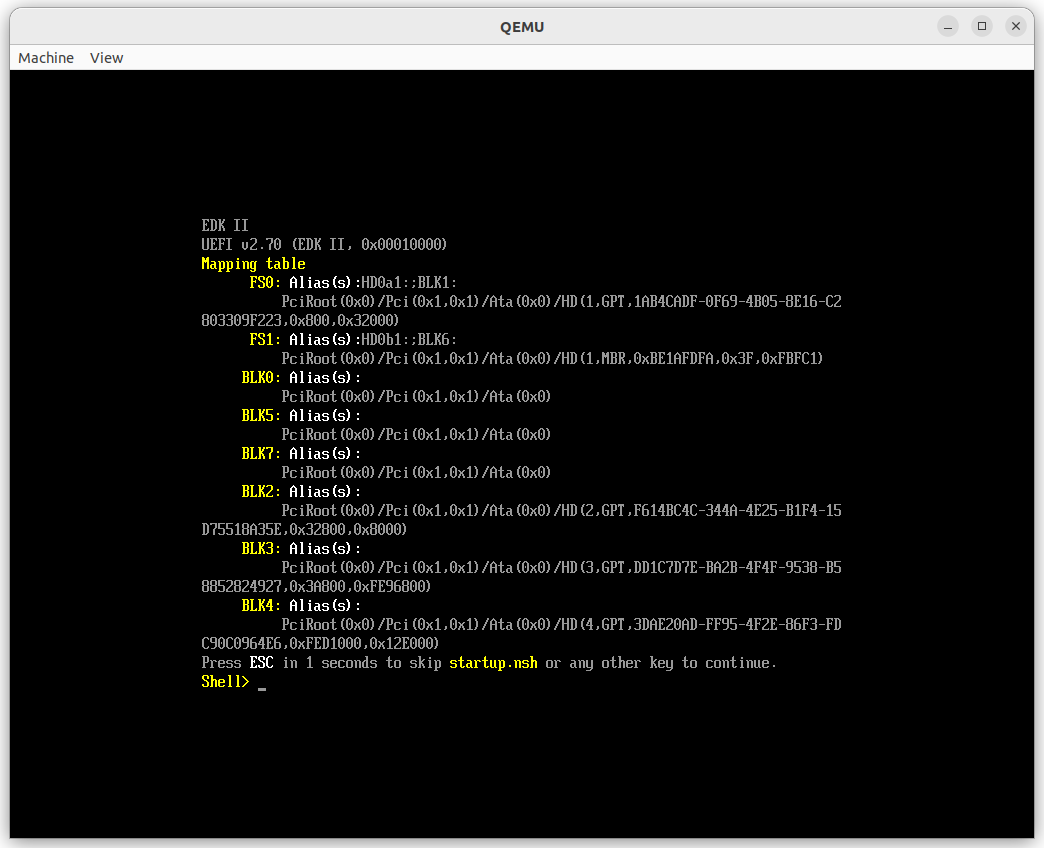
\includegraphics[width=1.0\textwidth]{attacks/neither/01_uefi_shell.png}
    \caption{\ac{UEFI} command prompt}
    \label{fig:uefi-shell}
\end{figure}


% showing mapping, also available with map command
% consistent device mapping, comparable to partition names in windows
The map command is very interesting for file access with the shell, it displays a mapping table between user defined alias names and device handles.
The aliases can be used instead of a device path when submitting commands via the command line interface.
The \ac{UEFI} shell also produces default mappings, notably for file systems \cite[3.7.2. Mappings]{uefi-shell-spec}.
These mappings are designed to be consistent across reboots as long as the hardware configuration stays the same, they are comparable to Windows partition letters \cite[Appendix A]{uefi-shell-spec}.

\TODO{find in spec what precise mapping mechanism}
When we inspect the mapping table we can see \lstinline{FSx:} and \lstinline{BLKx:} aliases, \lstinline{FSx:} maps to file systems and \lstinline{BLKx:} to block devices.
This identification is performed via instances of the \emph{Simple File System Protocol} and \TODO{double check} Block \ac{I/O} Protocol.
% explain Simple File System Protocol
The \emph{Simple File System Protocol} \cite[13.4 Simple File System Protocol]{uefi-spec} provides, together with the File Protocol, file-type access to the device it is installed on \cite[13.5 File Protocol]{uefi-spec}.
The two protocols are independent of the underlying file system the media is formatted with.


% load NtfsDxe.efi
Our \ac{NTFS} \ac{UEFI} Driver is one such abstraction and needs to be loaded, this is done by first entering the alias, for the file system containing the \lstinline{NtfsDxe.efi}.
This effectively switches the console's working directory to be the root of the entered file system, now we can invoke \lstinline{load} with the path to the executable.
The output indicates whether loading the driver was successful.
% drivers
% We can now list
With the command drivers, we can list all currently loaded drivers and some basic information about them, such as number of devices managed.
We can see that the NTFS driver already manages devices.

% map -r "reset all the default mappings in a system this option is useful if the system configuration has changed since the last boot"
% new mapping and fs ontop of old blk
We can now reset all default mappings with the map -r command to receive an updated list including the file systems now provided by the \ac{NTFS} driver.
The mapping also shows us that the file system now sits on top of a device which previously was only listed as a block device.

As done before we now type the alias of the new file system to switch to NTFS formatted file system.
With \lstinline{ls} we can list the current directory's content and confirm by the presence of the Windows folder that we are on the volume containing the Windows installation.
\TODO{maybe vol} % With \lstinline{vol} we can query information about the current volume, this shows us that our d


% navigate to Windows folder
% means read works
% try creating folder to test write
\TODO{Windows file access privileges}
We now navigate into the Windows folder to test whether we have unrestricted read and write access, since is not the case if done by an unprivileged user when performed from within Windows.
Accessing folders and viewing their contents is possible but creation of a new folder fails.

% debug why it failed
% find out its from windows having hibernation enabled by default
% change source code to not fallback to read only when encountering hibernation file
Upon debugging the \ac{NTFS} driver it appears to be that the drivers falls back to read only when it encounters a file that indicates that the Windows system is in hibernation mode.
Windows seems to have hibernation enabled by default and as such our rootkit should not rely on it being disabled, we can change the code of the \ac{NTFS} driver to not fallback when encountering this file.

We now know that provided we get to load the \ac{NTFS} driver we can access a Windows installation and subsequently the entire data of unencrypted hard drives.
Since our rootkit will not use the UEFI shell we need to have the \ac{NTFS} driver load as part of the boot process.

% try to use ntfs-driver in code
% this is our first rootkit iteration
% payload will also be DXE driver
% package payload in firmware image
The next step is for our bootkit to use the NTFS driver to gain file system access and write our payload to the Windows installation.
During our bootkit infection process we place the NTFS driver on the \ac{ESP}, so that our bootkit can load it.
In our bootkit, we can use the Loaded Image Protocol, that is installed to the handle of the bootkit's image in memory to retrieve the handle of the device our bootkit was loaded from \cite[9.1 EFI Loaded Image Protocol]{uefi-spec}.
This handle can then be used to call the Boot Services \lstinline{LoadImage} and \lstinline{StartImage} to load and execute the NTFS driver.
Since the driver conforms to the UEFI Driver Model, we need to also reconnect all controllers recursively, so it can assume controller over the NTFS formatted volumes, by installing the \emph{Simple File System Protocol} on their handles.
Loading the payload and other non-executable files into memory is done differently, here we use the handle from the Loaded Image Protocol to open the \emph{Simple File System Protocol} installed onto the \ac{ESP}, we can then call the \lstinline{OpenVolume} resulting in an instance of the File Protocol representing the root folder of the volume \cite[13.4]{uefi-spec}.
This instance can then be used to open and read our payload with the absolute path on the \ac{ESP} into memory.
% write payload
% seems to not be needed: install tag protocol on NTFS driver and put into depex of rootkit
% search for windows installation
% iterate over all \emph{Simple File System Protocol} instance
% open volume

\subsubsection{Payload deployment}

To perform the write operation we now need a handle we did not yet interact with, at least directly.
We can use the Boot Service \lstinline{LocateHandleBuffer} to receive an array of all handles that support the \emph{Simple File System Protocol}, this includes volumes such as the \ac{ESP} but also the Windows recovery partition.
We can iterate over all handles to open the volume and attempting to create a new file with a file path that's inside of the Windows installation.
This operation fails on volumes not containing a Windows installation which we can just skip.
Eventually the volume containing Windows is found and the file is created and opened successfully, we can then write our payload, that we read into memory earlier, onto the disk and close the file again.

Now the question arises as to where to write our payload to, we want automatic and elevated execution.
Earlier we discovered that the \ac{NTFS} \ac{DXE} driver disregards the file access permission model \TODO{Windows File Permissions} so we are not restricted in the same way an unprivileged user would be when accessing the disk.
\emph{MosaicRegressor} writes its payload to the Windows startup folder, a folder whose contents are automatically executed at system startup.
The programs within the startup folder are unfortunately not automatically run at an elevated level, so this isn't a suitable target location.

\TODO{DLL proxy loading}
\TODO{modifying Windows Executables KMCI}

% Task Scheduler
The Task Scheduler is a Windows service responsible for managing the automatic execution of background tasks \cite[10. The Task Scheduler]{windows-internals-7-part2}.
Tasks are performed on certain triggers, which may be time-based (periodically or on a specific time) or event-based, for example on user logon or system boot\cite{microsoft-task-scheduler-triggers}.
A task can perform various actions upon invocation \cite{microsoft-task-scheduler-actions}, but we will focus on command execution.
Most tasks will simply execute other programs as their action, this execution is performed under specified a security context \cite{microsoft-task-scheduler-security-contexts}.
The idea of our attack is to have a task, that performs its action with a high privilege level, execute our payload.
The task of our choosing is called \lstinline{Autochk\Proxy}, that performs the command

\begin{lstlisting}
%windir%\system32\rundll32.exe /d acproxy.dll,PerformAutochkOperations
\end{lstlisting}

30 minutes after system boot, the executable \lstinline{rundll32.exe} loads the \ac{DLL} \lstinline{acproxy.dll} and invokes the exported function \lstinline{PerformAutochkOperations} \cite{microsoft-rundll32}.
The function name as well as the task name suggest the performed action relates to the Windows utility \emph{autochk} which verifies the integrity of \ac{NTFS} file systems \cite{microsoft-autochk}.
The Task Scheduler keeps book of its active tasks in the registry under \lstinline{HKLM\SOFTWARE\Microsoft\Windows NT\CurrentVersion\Schedule\TaskCache}, grouped by four subkeys Boot, logon, plain and Maintenance.
These entries consist only of a \ac{GUID} that is used to look up the task descriptor saved under their respective task master (registry) keys, these task master keys are located under \lstinline{HKLM\SOFTWARE\Microsoft\Windows NT\CurrentVersion\Schedule\TaskCache\Tasks} \cite[10. The Task Scheduler - Initialization]{windows-internals-7-part2}.
There also exist a secondary copy of the task descriptors, on the regular file system under \lstinline{%windir%\system32\Task}, stored as \ac{XML} files.

We can use the Task Scheduler Configuration Tool to modify the target task on a system under our control, we change the executable path as well as remove the configured delay.
We then use the Windows registry editor \lstinline{reged.exe} to navigate to the task descriptor store, there we search for the task master key belonging to our task and export this key.

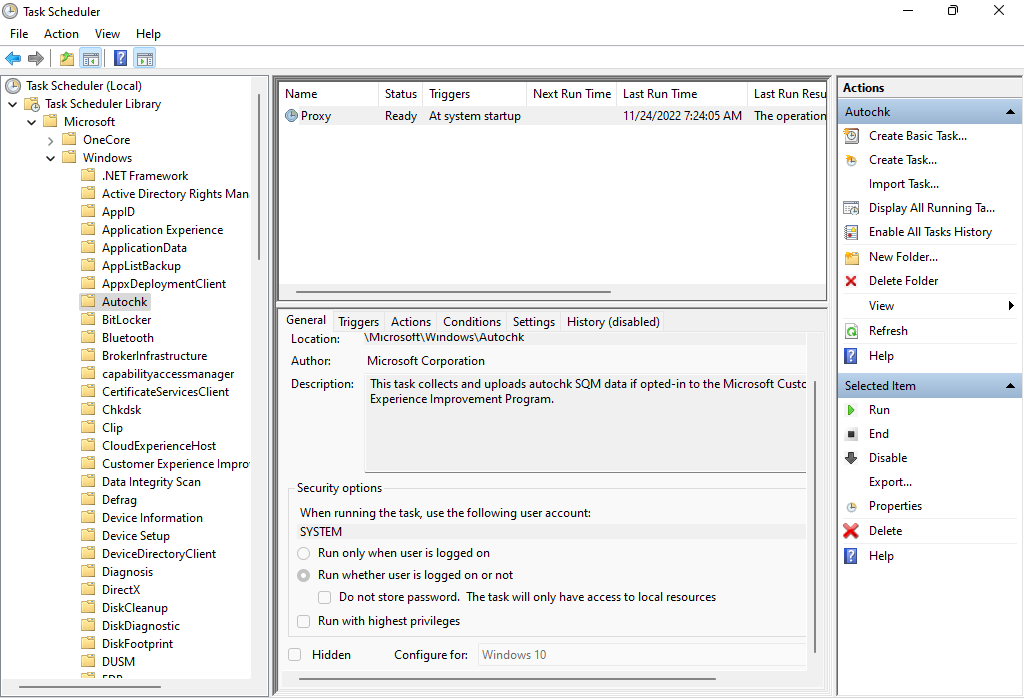
\includegraphics[width=\textwidth]{attacks/neither/05_taskscheduler_autochk.png}

% edit with start cmd.exe and trigger manually
% whoami
% We modify the task's action, to run our payload instead.
To verify the privileges our payload is executed with, we can save the output of \lstinline{whoami /all} into a file.
The \lstinline{whoami} command shows the current user and privileges \cite{microsoft-whoami}.
After manually triggering the task through the configuration tool, we see that our payload was run from the \lstinline{nt authority\system} user account, which is the most privileged system account \cite{microsoft-localsystem-account}.

% \TODO{whoami /all snippet}

% chntpw and reged
% edit Task in machine under Control
We can use this exported key and import it on our victim's system as part of our attack.
To import the key on an offline system, we can use a Linux utility called \lstinline{chntpw} whose primary purpose it is to reset the password of local windows user accounts \cite{chntpw}.
The library does this by editing the registry of a Windows installation and as such the author also offers a standalone registry editor called \lstinline{reged}.
% test
% dual boot
We can test the Linux tool when dual-booting a Linux and a Windows installation.
We place our payload in the Windows installation and then boot into Linux, where we can open the \lstinline{HKEY_LOCAL_MACHINE/SOFTWARE} hive in \lstinline{reged} and import our modified registry key.
% import and overwrite registry key on target machine
This overwrite the task descriptor and when booting into Windows our payload is executed.

% port to uefi
The next step is to port the \lstinline{reged} utility so that it works in the UEFI environment, so we can use it as part of our bootkit.
% most stdlib stuff is just mapping to UEFIlib stuff with equivalents or using gcc implementations
The porting process boils down to providing semantically equivalent definitions of external function calls, such as c standard library and Linux kernel functions, to link against.
Declarations and macros are still supplied by the local compiler's system headers.
Function definitions can often be translated to \ac{UEFI} equivalents, \ac{EDK} II has libraries offering implementations of commonly used abstraction.
% memory allocation (malloc, calloc, realloc), memory manipulation (memset, memcpy) string manipulation (sscanf, strtol), stdout (printf), abort, exit
Memory allocation maps to the MemoryAllocationLib, memory manipulation to BaseMemoryLib, basic string manipulation to BaseLib, stdout to PrintLib (only relevant for print debugging).
% cstdio is non trivial and has to be implemented by calling protocols on the right volume
Function calls related to standard input and output such as opening, reading and writing a file, namely the hive file, are more complex and have to be mapped to the \ac{UEFI} protocols \emph{Simple File System Protocol} and \emph{File Protocol}.
Luckily the author of \lstinline{reged} used distinct functions to access the hive file and registry file, making it possible to keep the original source code unmodified, except for a change in the import behavior.
The name of a task master key is the task's \ac{GUID}, which may differ from device to device, thus we cannot import a key into its exact path, we instead iterate over the subkeys of the target's parent key.
We then match for the name value of the key.

Now that we modified the Windows installation to execute our payload upon boot, we need to transfer execution from the bootkit to the original Windows Boot Manager.
Loading the original application is inspired by how the UEFI Boot Manger loads boot options, this includes relaying the \lstinline{LoadOptions} and \lstinline{ParentHandle} of the \emph{\ac{EFI} Loaded Image Protocol} \cite[9.1]{uefi-spec} instance installed to our bootkit to the Windows Boot Manager.


\subsection{Rootkit}

Performing the same attack in the form of a rootkit is very similar and mainly differs in the infection process.
The \ac{UEFI} payload is now compiled as a \ac{DXE} driver instead of an application.
When placed in the \ac{DXE} volume it is automatically loaded by the \ac{DXE} Dispatcher iterating over the \ac{FV}, loading  drivers whose dependencies are resolved.
The core functionality of our \ac{UEFI} payload is identical with the exception that we don't have to manually load the \ac{NTFS} driver anymore and accessing the Windows payload is now done with the \emph{Firmware Volume2 Protocol} defined in the \cite[3.4.1]{pi-spec}, instead of \emph{Simple Filesystem Protocol}. There are no traditional file names on a firmware volume, and we have to search for files using the module \acp{GUID}.

\subsubsection{Infection}

Infection with the rootkit is has a much higher barrier of entry, as it requires read and write access to the firmware image.
We have to retrieve the image, insert our payload in the \ac{DXE} volume and deploy the modified image.

\TODO{properly list the options}
This can be done by using a spi flash programmer and clamping the physical chip.
Or using an SPI chip emulator.
% for qemu we can build it ourselves
If we want to use emulation we can build the \ac{OVMF} Package from EDK II which is a firmware image for virtual machines.

Now that we have the image we can edit it with UEFITool, which is an editor for firmware images conforming to the \ac{UEFI} \ac{PI} specificatoin \cite{uefitool}.
In UEFITool we navigate to the \ac{DXE} Volume containing the \ac{DXE} Core and \ac{DXE} drivers.
% remove previous NTFS driver if present, for full control, might be read only etc
% in UEFITool search for string
Before adding our \ac{NTFS} driver we remove any other \ac{NTFS} driver that might already be packed in the image by \acp{OEM}, their version might be read-only or otherwise restricted and would inhibit our \ac{NTFS} driver from installing onto a device, if it were to load prior to ours.
UEFITool conveniently offers a function to search through the entire firmware image.
We can search for "NTFS" as a case-insensitive string, since most drivers either have a User Interface Section which contains a human-readable name for inspection tools like UEFITool \cite[Vol 3, 3.2.5]{pi-spec} or support the optional \emph{Component Name Protocol} which is part of the \ac{UEFI} Driver Model and returns the name of a driver \cite[11.5]{uefi-spec}.
If this were to not suffice it is possible to search for the \ac{NTFS} magic number indicating that a volume is formatted with \ac{NTFS}, this number is the string \ac{NTFS} encoded in \ac{ASCII} followed by four white spaces \lstinline{ 'N', 'T', 'F', 'S', ' ', ' ', ' ', ' '} and likely contained by an \ac{NTFS} driver.
% since files are part of file sections we cant drop in the .efi
We cannot directly drop our \ac{UEFI} payload in form of \lstinline{.efi} files with UEFITool, because \ac{DXE} drivers have three mandatory sections: the \ac{PE32} executable section, composed of the \lstinline{.efi} file content, a version section and the \ac{DEPEX} section \cite[Vol 3, 2.1.4.1.4]{pi-spec}.
% compile dxe driver within ovmf
% generate unused volume to receive .ffs file with version, depex, user interface and pe section
For our \ac{UEFI} payload to be generated as a sectioned \ac{FFS} file we add our files to the build process of \ac{OVMF} package in \ac{EDK} II. When part of the \ac{FDF} which is used to generate a firmware image file, the intermediary \lstinline{.ffs} files from the build process are of much value for us.
% pack executable binary as uefi module
% EDK II produces freeform image with one raw section
For our Windows payload we can use a special \ac{EDK} II module type which takes binary files as input, resulting in a sectioned file of type \lstinline{EFI_FV_FILETYPE_FREEFORM}, with no restrictions on the contained file sections \cite[Vol 3, 2.1.4.1.7]{pi-spec}.
The output contains only one file section of type \lstinline{EFI_SECTION_RAW} consisting of the binary payload.
This use of this special module has the benefit that its \ac{GUID} is used to attribute the sectioned file when being placed in the firmware volume.
Not that we have \lstinline{.ffs} files corresponding to all our resources used in the attack we can import these into the target image with UEFITool.

\TODO{this}
overwrite the SPI flash with modified image by using the programmer again.